%!TEX root = ../dd.tex
\pagebreak
\section{User Interface Design}
\label{sec:ui}
This section briefly illustrates the design behind the UI for the main app and the taxi driver app. In order to accomplish this, two UX diagrams are provided:
\begin{itemize}
    \item The first one represents the structure of the taxi driver's mobile app. A much simpler interface is provided (mainly for two operations: accept/refuse request and obtain directions towards destination). 
	\item The second one represents the structure of the official mobile and web app. Each screen gives the possibility to use a main functionality (request a taxi, reserve one, sign up...). For a visual representation of each screen, please refer to the RASD document.
	
\end{itemize}

\begin{figure}[bth]
    \centering
    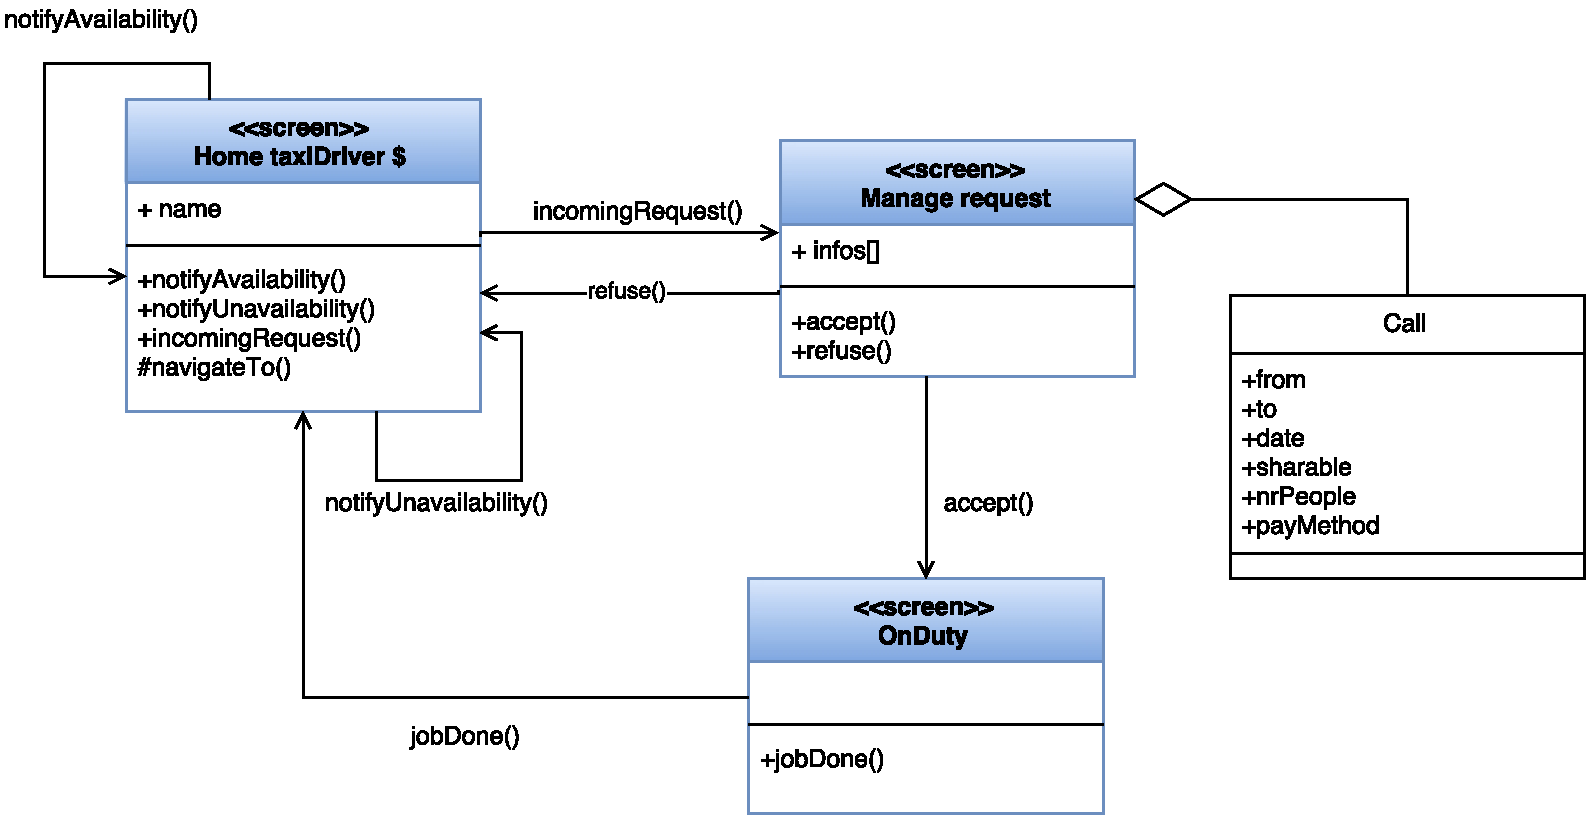
\includegraphics[width=0.85\textwidth]{UXTDriver}
    \caption{UX for driver app}
    \label{fig:ux2}
\end{figure}

\begin{figure}
    \centering
    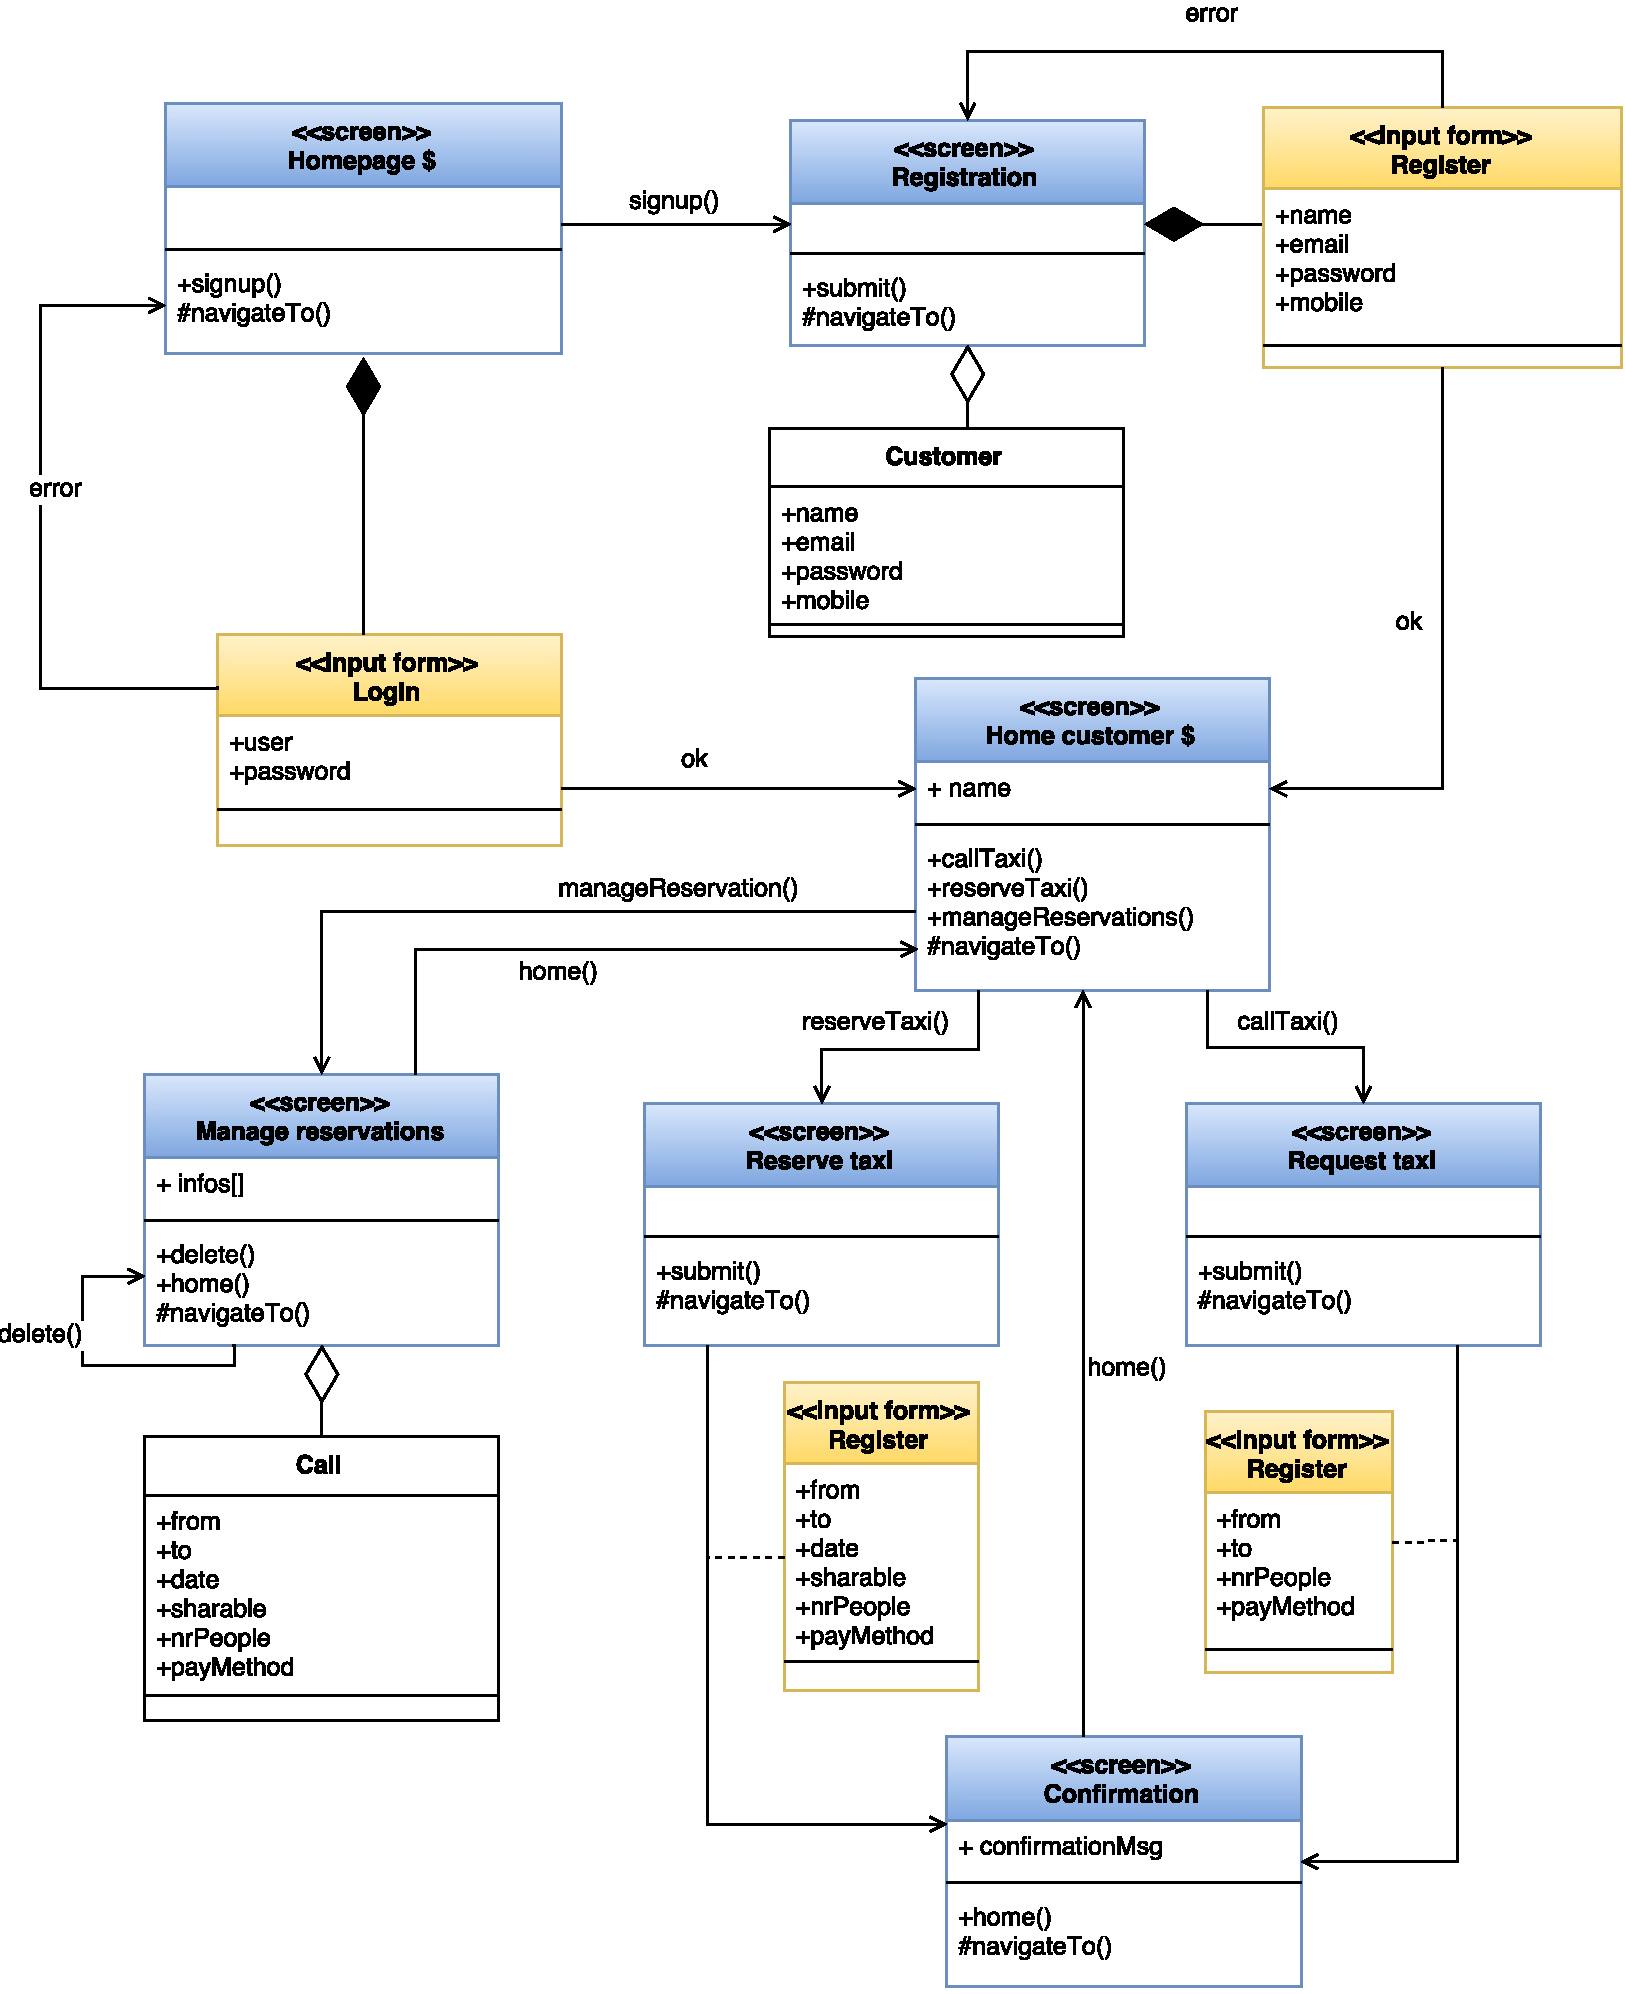
\includegraphics[width=0.85\textwidth]{UX}
    \caption{UX for main application}
    \label{fig:ux1}
\end{figure}

